%% Based on a TeXnicCenter-Template by Gyorgy SZEIDL.
%%%%%%%%%%%%%%%%%%%%%%%%%%%%%%%%%%%%%%%%%%%%%%%%%%%%%%%%%%%%%

%------------------------------------------------------------
%
\documentclass[letterpaper,10pt]{article}%
%Options -- Point size:  10pt (default), 11pt, 12pt
%        -- Paper size:  letterpaper (default), a4paper, a5paper, b5paper
%                        legalpaper, executivepaper
%        -- Orientation  (portrait is the default)
%                        landscape
%        -- Print size:  oneside (default), twoside
%        -- Quality      final(default), draft
%        -- Title page   notitlepage, titlepage(default)
%        -- Columns      onecolumn(default), twocolumn
%        -- Equation numbering (equation numbers on the right is the default)
%                        leqno
%        -- Displayed equations (centered is the default)
%                        fleqn (equations start at the same distance from the right side)
%        -- Open bibliography style (closed is the default)
%                        openbib
% For instance the command
%           \documentclass[a4paper,12pt,leqno]{article}
% ensures that the paper size is a4, the fonts are typeset at the size 12p
% and the equation numbers are on the left side
%
\usepackage{amsmath}%
\usepackage{amsfonts}%
\usepackage{amssymb}%
\usepackage{graphicx,color}

\oddsidemargin=0.0in
\evensidemargin=0.0in
\textwidth=6.5in
\headheight=0.25in
\topmargin=0.0in
\textheight=8.5in


%-------------------------------------------
\newtheorem{theorem}{Theorem}
\newtheorem{acknowledgement}[theorem]{Acknowledgement}
\newtheorem{algorithm}[theorem]{Algorithm}
\newtheorem{axiom}[theorem]{Axiom}
\newtheorem{case}[theorem]{Case}
\newtheorem{claim}[theorem]{Claim}
\newtheorem{conclusion}[theorem]{Conclusion}
\newtheorem{condition}[theorem]{Condition}
\newtheorem{conjecture}[theorem]{Conjecture}
\newtheorem{corollary}[theorem]{Corollary}
\newtheorem{criterion}[theorem]{Criterion}
\newtheorem{definition}[theorem]{Definition}
\newtheorem{example}[theorem]{Example}
\newtheorem{exercise}[theorem]{Exercise}
\newtheorem{lemma}[theorem]{Lemma}
\newtheorem{notation}[theorem]{Notation}
\newtheorem{problem}[theorem]{Problem}
\newtheorem{proposition}[theorem]{Proposition}
\newtheorem{remark}[theorem]{Remark}
\newtheorem{solution}[theorem]{Solution}
\newtheorem{summary}[theorem]{Summary}
\newenvironment{proof}[1][Proof]{\textbf{#1.} }{\ \rule{0.5em}{0.5em}}

\begin{document}

\title{Compiling GMAT using Visual Studio 2010\\\textit{Express Edition Instructions}}
\author{Darrel J. Conway\thanks{Support provided by NASA GSFC FDSS Contract, Task 28.}
\\Thinking Systems, Inc.\\Tucson, AZ}
\date{March 2011}
\maketitle

\begin{abstract}
This document describes the steps needed to build GMAT using Visual Studio 2010, Express Edition (VS2010).  The instructions start with a fresh installation of VS2010, provide directions for installing wxWidgets, and finally for building GMAT. 
\end{abstract}

\section{Introduction}

The General Mission Analysis Tool, GMAT, is a space trajectory optimization and mission analysis system developed by NASA and private industry in the spirit of the NASA Vision. GMAT contains new technology and is a testbed for future technology development. To satisfy NASA's mandate and maximize technology transfer, GMAT is an open source software system licensed under the NASA Open Source Agreement.  Interested parties are encouraged to use GMAT to plan spacecraft missions, to build the system when they have requirements for features not yet included in GMAT, and to contribute new capabiliities to the system either through direct contributions to the code base or through plugin libraries.

This document describes the steps a new developer takes to set up a build environment for GMAT using Microsoft's Visual Studio development system.  The instructions were written using Visual Studio 2010 Express Edition, and validated using bot the Express Edition and the Professional Edition.  The following instructions assume that the developer is running a Windows XP, Vista, or Windows~7 based computer.  Separate instructions are available for users building GMAT with the Gnu Compiler Collection (gcc) on Windows, Mac, or Linux based computers.

The following sections describe installation of the compiler, folder arrangements and code used in the GMAT build files, preliminary steps necessary to collect and build the libraries GMAT needs, and the build steps for GMAT itself.  The document concludes with instructions for plugin libraries that GMAT uses to interface with MATLAB and the MATLAB Optimization toolbox, to perform estimation (the estimation plugin is a preview of capabilities still in development), and the VF13ad optimizer (core code available separately).

\section{Installing Visual C++ 2010 / Visual Studio 2010 Express Edition}

The Visual C++ environment can be installed either fron a web-based installer or from disk.  Users of the paid versions of Visual C++ should skip this section and install the product following the instruction provided by Microsoft.  Users of the Express edition can install from the onlins instructions provided by Microsoft, or by following the instructions provided here.

\subsection{Option 1: Web installation}

Visual C++ can be installed using a web based installer by following these steps:

\begin{enumerate}
	\item Open a web browser and browse to the Visual Studio 2010 Express download page: \\http://www.microsoft.com/express/Downloads/\#2010-Visual-CPP
	\item Download the installer for Visual C++
	\item Open the installer (vc\_web.exe) by double clicking on it
	\item Follow the installation instructions
\end{enumerate}

\subsection{Installing from a Disk Image}

If you have a disk containing Visual Studio Express, follow these steps:

\begin{figure}
\centering

\includegraphics{DiskStart.eps}
\caption{Screen for a New Disk}
\label{fig:DiskStart}
\end{figure}

\begin{figure}
	\centering
		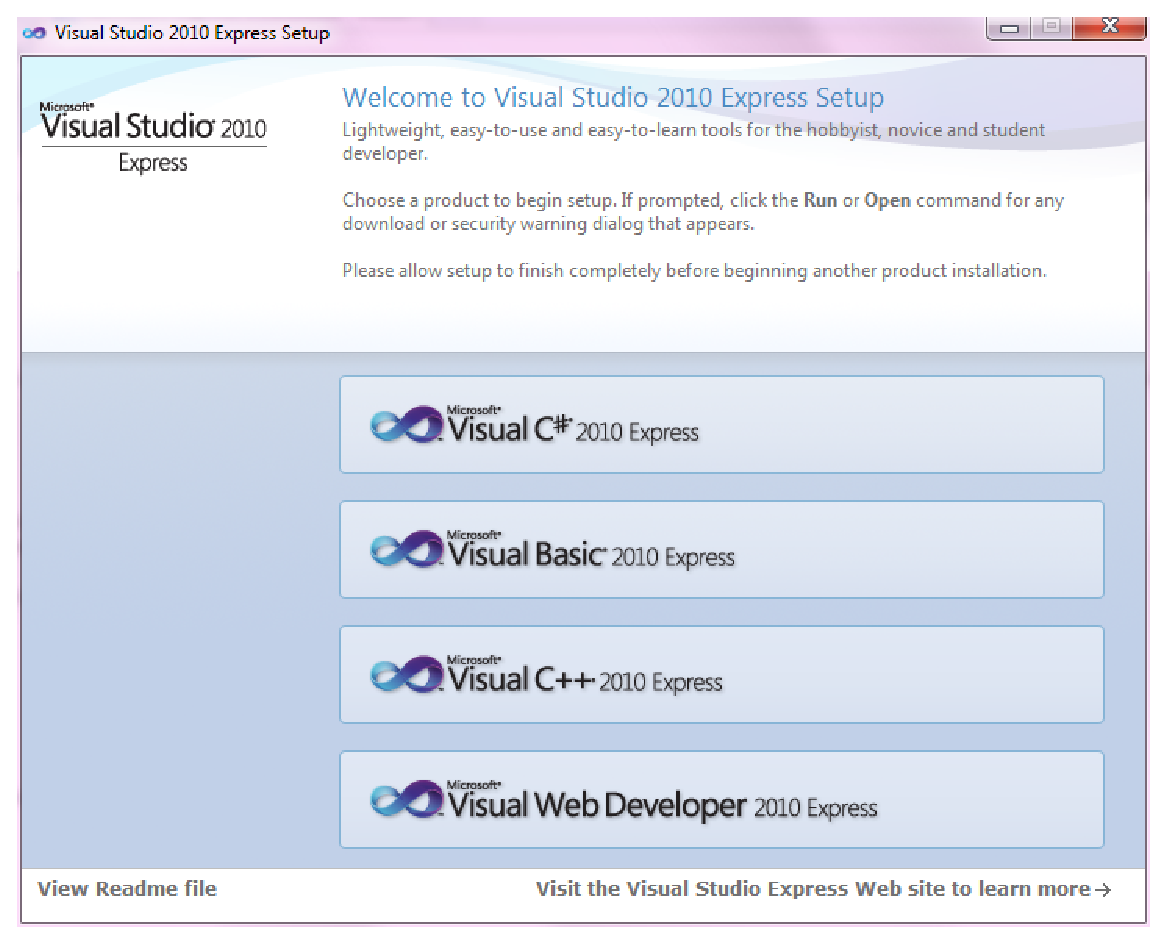
\includegraphics[height=4in,width=6in,keepaspectratio]{VisualCpp.eps}
	\caption{To add: Select Visual C++ Here}
	\label{fig:VisualCpp}
\end{figure}

\begin{enumerate}
\item Put the installation disk into your DVD drive
\item If prompted, select ``Run Setup.hta'' from the Autoplay Menu (See Figure~\ref{fig:DiskStart})
\item Select Visual C++ 2010 Express from the menu that opens (See Figure~\ref{fig:VisualCpp})
\item Follow the installation instructions.  GMAT does not require SQLServer, so you can deselect that option for installation.
\end{enumerate}

\subsection{64-bit Compilers (Optional)}

If you plan to build the 64-bit version of GMAT, you'll need to install the Windows 7 SDK version 7.1.  You'll also need to be running on a 64-bit version of Windows so you can test the resulting build.

The SDK can be downloaded from (all on one line)
\begin{quote}
\begin{verbatim}
http://www.microsoft.com/downloads/en/details.aspx?FamilyID=6b6c21d2-2006-4afa-
9702-529fa782d63b\&displaylang=en
\end{verbatim}
\end{quote}
\noindent Download the web based installer by clicking on the ``Download'' button, and then run it.  This installs the software development kit, including a 64-bit compiler.

\section{Folder Configuration}

Create a folder for building GMAT.  I'll use C:\textbackslash GmatVS as the root folder in this document.  This folder will contain the subfolders for third party components of the build -- wxWidgets, cspice, pcrecpp, and similar files.  Add the following folders to your root folder:
\begin{itemize}
\item Gmat3rdParty
\item GmatDevelopment
\item GmatPlugins (if you will be using the configuration managed plugin libraries)
\end{itemize}

\noindent Inside of the Gmat3rdParty folder, create the following subfolders; for the 32-bit builds:
\begin{itemize}
\item cspice
\item f2c
\item pcre
\item wxWidgets
\end{itemize}

\begin{figure}
\centering
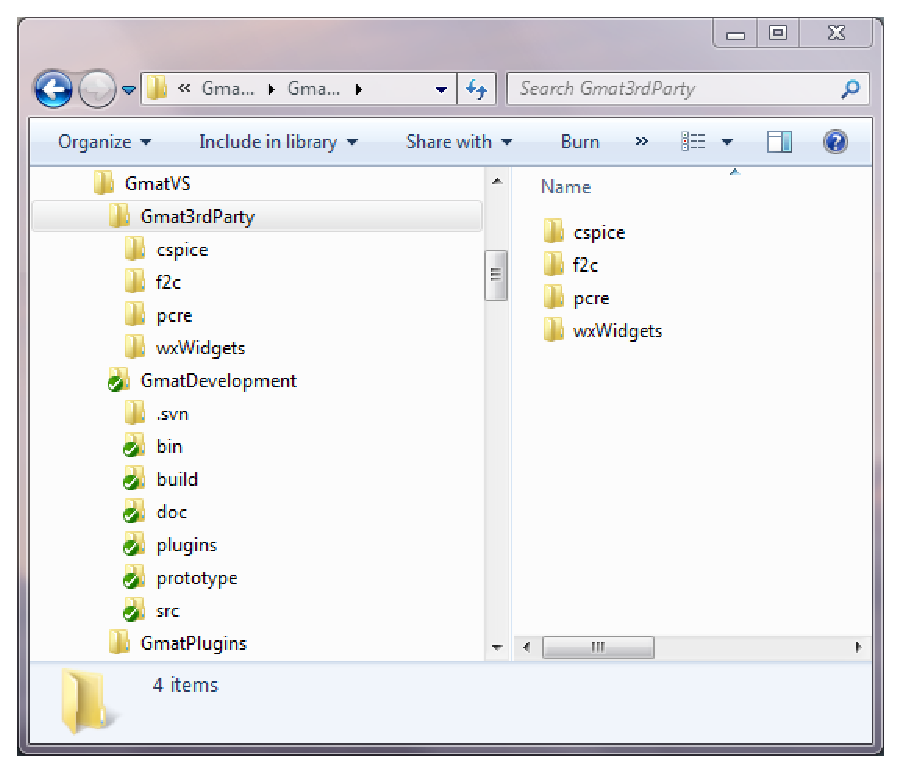
\includegraphics{FolderStructure.eps}
\caption{The File Structure used in GMAT's Conguration Managed Build Files}
\label{fig:FolderStructure}
\end{figure}


\noindent At this point, your folder structure should match the structure shown in Figure~\ref{fig:FolderStructure}.  If you want to also build the 64-bit release and have either a paid version of Visual Studio 2010 (that is, Professional, Premium, or Ultimate), or, if you installed the 64-bit tools in the Windows SDK so you can build a 64-bit version of GMAT, add these folders for the 64-bit versions of the 3rd party tools:
\begin{itemize}
\item cspice64
\item f2c64
\item pcre64
\item wxWidgets64
\end{itemize}

\section{Downloading GMAT}

GMAT's source code is located in a Subversion repository at SourceForge.  In addition to the source code, the repository at SourceForge contains the build files we'll need to proceed, including wxWidgets project files configured for Visual Studio 2010.  Because of this, you need to begin by downloading the GMAT development code using a Subversion client.  I am using SmartSVN on Windows, but any client should work.  Set up your client to access code at the following URL:

\begin{quote}
https://gmat.svn.sourceforge.net/svnroot/gmat/trunk
\end{quote}
\noindent Check out the entire source tree from that location.  When you check out the tree from this location, you'll retrieve GMAT's source code, development files, documentation, source for several plugin libraries, and the support files needed to run GMAT. 

\section{Building wxWidgets}

From this point through Section~\ref{sec:Plugins} we will concentrate on the 32-bit build of GMAT.  Appendix~\ref{app:64bit} describes the settings and changes necessary to build GMAT as a 64-bit application.  We begin by building wxWidgets, the GUI toolkit used for GMAT's user interface.

\subsection{Install the wx Code}

\begin{enumerate}
\item Download wxWidgets 2.8 from http://wxwidgets.org/downloads/.  Use the latest stable version of the 2.8 tree (2.8.12 at this writing), and download the wxMSW package.
\item Unpack the wx code into the folder named wxWidgets in your Gmat3rdParty folder.  You should see folders named art, build, contrib, demos, docs, include, lib, locale, samples, src, and utils in the wxWidgets folder when finished.
\item Visual Studio 2010 has trouble processing the Visual C++ project files that ship with wx.  Instead, we'll use files already configured (using Visual Studio 2010 Professional) for wx at Thinking Systems. 
\begin{enumerate}
\item The Visual Studio 2010 solution and project files for wxWidgets are located in an archive file in the GMAT folders you checked out earlier.  Find the file wxmsw.zip in the build\textbackslash GmatVS2010 folder of that working copy of the code.
\item Unpack the wxmsw.zip archive into your wxWidgets\textbackslash build\textbackslash msw folder.
\item Check to see that the file wx\textbackslash dll.sln is in your Gmat3rdParty\textbackslash wxWidgets\textbackslash build\textbackslash msw folder.  If, instead, you see that there is a folder named wxmsw in that folder, move its contents into the Gmat3rdParty\textbackslash wxWidgets\textbackslash build\textbackslash msw folder. 
\end{enumerate}
 
\end{enumerate}

\subsection{Prepare and Build wxWidgets}
\begin{enumerate}
\item Open Visual Studio
\item Select ``File | Open | Project/Solution...'' from the menu bar
\item Open the wx\textbackslash dll.sln solution file from the build\textbackslash msw folder of your wxWidgets installation.  (For me, the file is found in  C\:\textbackslash GmatVS\textbackslash Gmat3rdParty\textbackslash wxWidgets\textbackslash build\textbackslash msw)
\item GMAT needs the wxWidgets OpenGL components as part of the build.  This is configures in the wx\textbackslash setup.h configuration file for the build.  We need to change a setting in this file from its default setting.
\begin{enumerate}
	\item Open one of the projects in the Visual Studio solution tree
	\item Open the Setup Headers folder in this project
	\item Open the first setup.h file in the folder by double clicking on it
	\item If this file has the line ``\textbackslash\textbackslash  Name:        wx/univ/setup.h'' at the top, open the other setup file. (You want to edit the file in msw rather than in univ; the file you want identifies itself as ``wx/msw/setup.h''.)
	\item Search for wxUSE\_GLCANVAS in the open file
	\item Set wxUSE\_GLCANVAS to 1 rather than the default value of 0
	\item Save and close the file.
\end{enumerate}
\item On the Visual C++ toolbar select ``DLL Release'' (specifying the build configuration) and set your solution platform to Win32.  Figure~\ref{fig:wxSettings} shows these settings.
\item Build the solution (right click on the ``Solution 'wx\_dll'{}'' node at the top of the tree and select ``Build Solution''.)
\item Most, but not all, of the solution will build.  You may need to repeat the build process to get all of the libraries GMAT requires built.  Build the solution again until all but the dbgrid projects build.  (You are done when 19 of the 20 projects build.)
\end{enumerate}

\begin{figure}
\centering
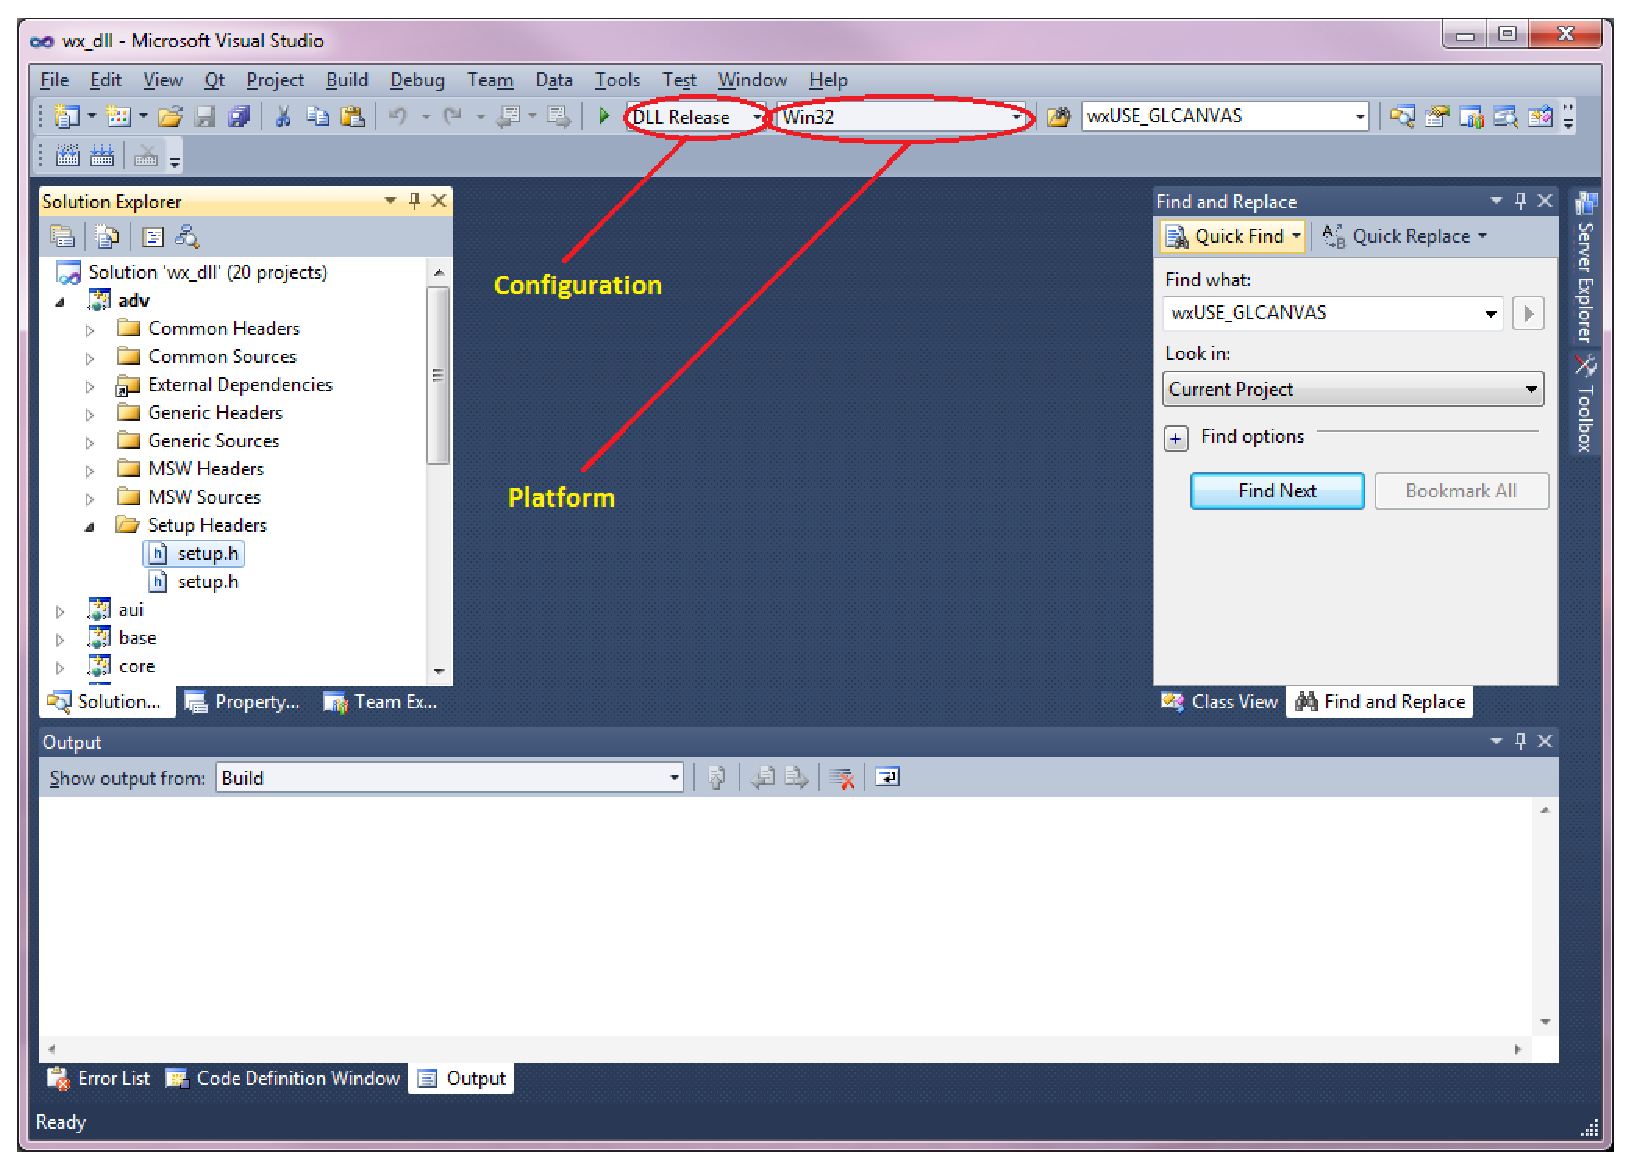
\includegraphics[scale=0.6]{DLLRelease.eps}
\caption{Configuration and Platform Settings for the 32-bit wxWidgets Build}
\label{fig:wxSettings}
\end{figure}

\noindent Check to see that you have 13 dll files in the wxWidgets\textbackslash lib\textbackslash vc\_dll folder.  Copy these into your GmatDevelopment/application/bin folder.

\section{Preparing SPICE (Optional)}

GMAT can be built to include readers and writers for data in the SPICE kernel format supplied by the Jet Propulsion Laboratory (JPL).  If you want to build GMAT with these extensions, follow these steps:

\begin{enumerate}
\item Download the SPICE toolkit for Visual C.  The 32-bit edition is available from
\begin{quote}
http://naif.jpl.nasa.gov/naif/toolkit\_C\_PC\_Windows\_VisualC\_32bit.html
\end{quote}
\noindent and the 64-bit version from
\begin{quote}
http://naif.jpl.nasa.gov/naif/toolkit\_C\_PC\_Windows\_VisualC\_64bit.html
\end{quote}
\noindent You want the file named cspice.zip.
\item Unpack the archive into your Gmat3rdParty\textbackslash cspice (or cspice64 for 64-bit) folder.  You should unpack the files so that you have, for example, a Gmat3rdParty\textbackslash cspice\textbackslash include folder that contains the cspice header (.h) files.  
\end{enumerate}

\noindent Note that cspice includes the Fortran to C library code; if you build with SPICE, you do not need to manage f2c separately when working with the GMAT base library code.

\section{Preparing f2c (Optional)}

GMAT uses the Fortran to C compiler, f2c, for certain dynamics models and solvers.  The SPICE libraries from JPL include the f2c library code as part of their library.  If you plan to work exclusively with GMAT's source code using a build that includes the SPICE extensions and do not have Fortran code that you need to convert to C, you can skip this step.  Otherwise, you need to follow these steps to configure the f2c system:

\begin{enumerate}
\item A minimal f2c build is contained in the archive f2c.zip, located in the GmatDevelopment\textbackslash build\textbackslash windows-VS2010 folder.  Locate this file.
\item Unpack the file into your Gmat3rdParty\textbackslash f2c folder.  You should have three directories as a result: Gmat3rdParty\textbackslash f2c\textbackslash bin, Gmat3rdParty\textbackslash f2c\textbackslash lib, and Gmat3rdParty\textbackslash f2c\textbackslash include, along with a file containing the copyright notice of the owners of the f2c system.
\end{enumerate}

This completes installation of f2c.  The full source for the system can be downloaded and built from http://www.netlib.org/f2c/.

\section{Building GMAT}

At this point, GMAT should build without further configuration.  Follow these steps:
\begin{enumerate}
\item Open Visual C++
\item Select ``File | Open | Project/Solution...'' from the menu bar
\item Browse to the GmatDevelopment\textbackslash build\textbackslash GmatVS2010 folder
\item Select the GmatVS2010.sln solution file and click the Open button.  The GMAT solution will open and show projects to build GMAT and several plugin libraries.
\item The solution has several configurations, depending on how you want to proceed: Debug, ReleaseWithoutF2C, Release, and ReleaseWithSPICE.  Here's what you need to know about them:
\begin{itemize}
\item \textbf{Debug}:  A build with full debug enabled.  This build runs quite slowly, and is not recommended for general use, but may be helpful when debugging the system.  It does not use either SPICE or the MSISE90 model.
\item \textbf{ReleaseWithoutF2C}: This configuration builds a working GMAT, but the MSISE90 code is turned off.  You might want to build it first, to test your setup.
\item \textbf{Release}: Includes an f2c'd version of MSISE90 enabled; you'll need f2c installed in the locations described above to use this configuration.
\item \textbf{ReleaseWithSPICE}: This is the "Guaranteed to work" configuration of GMAT that includes all of the base components, and includes the plugin libraries for MATLAB and the fmincon optimizer.  Note that the MATLAB extensions require additional configuration, described below.
\end{itemize}
\item Set the configuration to ReleaseWithoutF2C, Release, or ReleaseWithSPICE, depending on the elements installed in previous sections.
\item Right click on the GMAT\_wxGui project, and select Rebuild to completely build GMAT.  This process takes a few minutes.  
\item Open a windows explorer and browse to your GmatDevelopment\textbackslash bin folder.  You should see GMAT.exe there, along with libGmatBase.dll and your wxWidgets libraries.
\item Set up the GMAT data files and other files needed to run GMAT (See Appendix A).
\item Double click on the GMAT.exe file to run GMAT.  Press the Run button to run the default mission.  Rejoice.
\end{enumerate}

\section{Building the MATLAB Plugin Libraries for MATLAB and fmincon (Optional)}

Next we will build the GMAT MATLAB interface.  You'll need to have MATLAB installed to build the MATLAB interface, and you'll also need the Optimization Toolbox to build the fmincon optimization plugin.

\begin{figure}
	\centering
		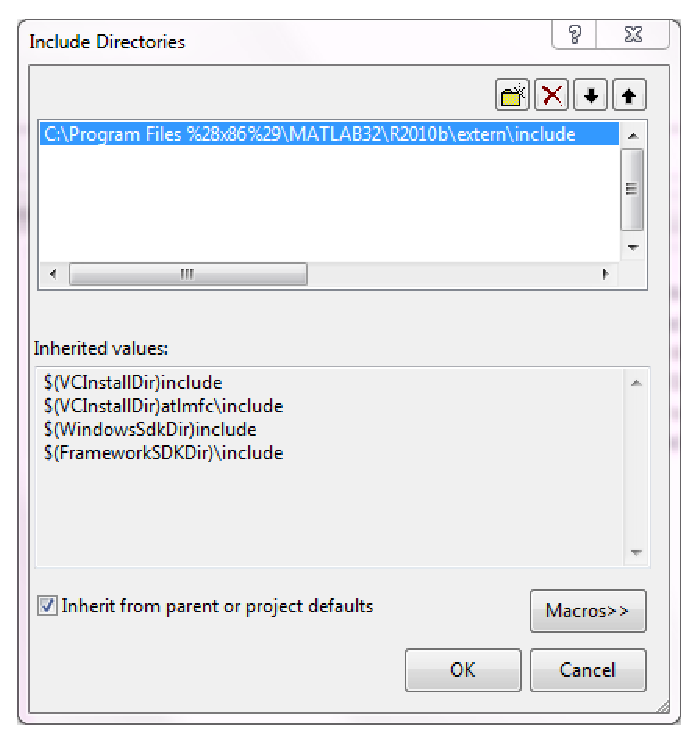
\includegraphics{SettingIncludeFolder.eps}
	\caption{MATLAB Include Settings}
	\label{fig:SettingIncludeFolder}
\end{figure}


\begin{enumerate}
\item Open Visual C++
\item Select ``File | Open | Project/Solution...'' from the menu bar
\item Browse to the GmatDevelopment\textbackslash build\textbackslash GmatVS2010 folder
\item Select the GmatVS2010.sln solution file and click the Open button.  The GMAT solution will open and show projects to build GMAT and several plugin libraries.
\item Set your include and library paths for the libMatlabInterface and libFminconOptimizer projects.  This is done by following these steps for each project:
\begin{enumerate}
\item Right click on the project node (either libMatlabInterface or libFminconOptimizer)
\item Select the ``Properties'' entry on the pop-up menu
\item On the dialog that appears, set the Configuration to ``All Configurations''
\item Select the ``Configuration Properties | VC++ Directories'' entry on the property tree in the left panel of the dialog
\item Select the ``Include Directories'' line, and select <Edit...> from the drop-down button that sets the directory list
\item A new dialog appears that lists the include directory settings for at the project scope.  Click on the first entry in the list, and then click on the button to its right labeled with ellipses (...)
\item A file browser will appear.  Navigate in this browser to your MATLAB folder, and then inside of it, navigate to the ``extern\textbackslash include'' folder.  This folder contains the header files GMAT needs to build the interface.  Click the ``Select Folder'' button to select it.  
\item Once the file browser window closes, your include dialog should resemble the one shown in Figure~\ref{fig:SettingIncludeFolder}.  Press the OK button.
\end{enumerate}
\item Right click on the libMatlabInterface project, and select Build.  (Don't select Rebuild unless you want to also rebuild libGmatBase.dll).
\item Right click on the libFminconOptimizer project, and select Build.  (Don't select Rebuild unless you want to also rebuild libGmatBase.dll and libMatlabInterface).
\item \textit{Sketchy, needs to be filled in} Add the new libraries to your GMAT startup file
\item Open a windows explorer and browse to your GmatDevelopment\textbackslash bin folder.  You should see libMatlabInterface.dll and libFminconOptimizer.dll in the folder now.
\item Double click on the GMAT.exe file to run GMAT.
\item \textit{Sketchy, needs to be filled in} Check to confirm that fmincon is now available as an optimizer.
\end{enumerate}


\section{\label{sec:Plugins}Standard GMAT Plugins}

There are four standard plugin libraries that are built for GMAT at this writing.  If you have access to the plugin repositories, you can configure and build these optional libararies: libDataFile, libCcsdsEphemerisFile, libGmatEstimation, and libVF13Optimizer.  The VF13ad optimizer library and the Estimation library both use the Fortran to C library, so if you plan to build those components, follow the steps above to build f2c.  The DataFile pluging and the CcsdsEphemerisFile plugin use the C++ extensions to the Perl Compatible Regular Expression library, pcrecpp.  Configuration of that component is described next.

\subsection{Configuring ang Building PCRECPP (Optional)}

GMAT uses the C++ version of the Perl Compatible, pcrecpp, for string manipulation when working with data files and CCSDS based ephemeris products.  The following steps describe how to set up pcrecpp.

\begin{enumerate}
\item Download the pcre 8.12 (to guarantee project file consistency -- preassembled Visual C++ 2010 solutions are packaged in the GMAT repository; other versions may require some modification to the build configuration) from ftp://ftp.csx.cam.ac.uk/pub/software/programming/pcre/
\item Unpack the download into your Gmat3rdParty/pcre folder.  This will give you a folder named pcre-<version>, where <version> is the version number for the library.  (For me, the resulting folder is Gmat3rdParty/pcre/pcre-8.12.)
\item Copy the contents of pcre-8.12 into the pcre folder, moving them up one level.  This places the header files in teh location needed to build the plugins.
\item The usual way to build pcre is to download and install CMake for your platform, use it to create build files (Makefiles on unix like systems, project files and solution files on Windows), and then build from those files. The pcre library files have already been created for pcre-8.12, and can be found in the GMAT plugins build folder build\textbackslash windows-VS2010 in the archive pcre-VS2010-out.zip.
\item Locate pcre-VS2010-out.zip.
\item Unpack its contents into your pcre folder.  This will create a lib and a dll folder in your pcre folder.
\item Copy the contents of the pcre\textbackslash dll folder into your GMAT executable folder.
\end{enumerate}

This completes the pcre setup.  If you'd prefer to compile pcre yourself, the instructions for doing this using CMake can be found in the pcre\textbackslash NON-UNIX-USE file.  Just be sure that you place the resulting libraries in place in pcre\textbackslash lib and pcre\textbackslash dll.

\begin{thebibliography}{9}                                                                                               
\bibitem {VisualStudio} Visual Studio Express can be downloaded from http://www.microsoft.com/express/Downloads/\#2010-Visual-CPP

\bibitem {wx} http://wxwidgets.org/downloads/

\bibitem {spice} http://naif.jpl.nasa.gov/naif/index.html

\end{thebibliography}


\appendix

\section{GMAT Data Files and Support Files }

\textit{Here I'll describe the files folder, etc}

\section{\label{app:64bit}Building GMAT in 64-bit mode}

\textit{To be written}

\end{document}
